\documentclass[border=2pt]{standalone}
\usepackage{times}
\usepackage{amsmath,amssymb}
\usepackage{tikz}
\usetikzlibrary{arrows.meta,calc,positioning}
\begin{document}
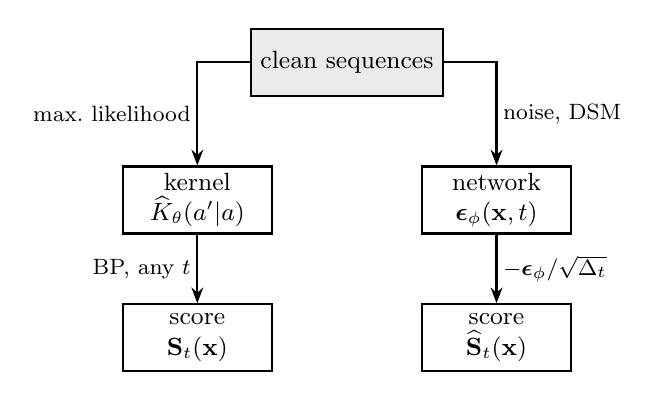
\begin{tikzpicture}[
    box/.style={draw,thick,align=center,font=\small,minimum height=8.5mm,inner sep=2pt,text width=1.75cm},
    data/.style={box,fill=black!8,text width=2.3cm},
    arr/.style={-{Stealth[length=2mm]},thick},
    lab/.style={font=\footnotesize,align=center,inner sep=2pt}]
  \node[data] (a) at (0,0) {clean sequences};
  \node[box] (k) at (-1.9,-1.75) {kernel\\ $\widehat K_\theta(a'|a)$};
  \node[box] (n) at (1.9,-1.75) {network\\ $\boldsymbol{\epsilon}_\phi(\mathbf{x},t)$};
  \node[box] (s1) at (-1.9,-3.5) {score\\ $\mathbf{S}_t(\mathbf{x})$};
  \node[box] (s2) at (1.9,-3.5) {score\\ $\widehat{\mathbf{S}}_t(\mathbf{x})$};
  \draw[arr] (a.west) -| node[lab,left,pos=0.75]{max.\ likelihood} (k.north);
  \draw[arr] (a.east) -| node[lab,right,pos=0.75]{noise, DSM} (n.north);
  \draw[arr] (k) -- node[lab,left]{BP, any $t$} (s1);
  \draw[arr] (n) -- node[lab,right]{$-\boldsymbol{\epsilon}_\phi/\sqrt{\Delta_t}$} (s2);
\end{tikzpicture}
\end{document}
